\documentclass[14pt]{extarticle}
\usepackage{fontspec}
\usepackage{polyglossia}
\usepackage{amsmath}
\usepackage{amssymb}
\usepackage{xcolor}
\usepackage{fancyhdr}
\usepackage{graphicx}
\usepackage{listings}
\usepackage[most]{tcolorbox}
% \usepackage{setspace}
\usepackage{pifont}
\usepackage{enumitem}
\usepackage{titlesec}
\usepackage[bottom]{footmisc}
\usepackage{titling}
\usepackage{minted}
\usepackage{etoolbox}
\usepackage{array}
\usepackage{extsizes}
\usepackage{float}
\usepackage{booktabs}
\usepackage{hyperref}
\usepackage[onehalfspacing]{setspace}
\newif\ifcolorblind
\ifdefined\setcolorblind
  \setcolorblind
\fi

\ifcolorblind
  \usepackage[a4paper, landscape, top=1cm, bottom=1cm, left=1cm, right=1cm, headheight=1.5cm, headsep=0.5cm]{geometry}
\else
  \usepackage[a4paper, top=2.7cm, bottom=2.7cm, left=2.5cm, right=2.5cm, headheight=1.5cm, headsep=0.5cm]{geometry}
\fi
\usepackage{tikz}
\usepackage{datetime2}

\usetikzlibrary{automata, positioning, arrows.meta, arrows}

\newfontfamily\emoji{Segoe UI Emoji}

\pagestyle{fancy}

\setmainlanguage[numerals=western]{arabic}
\setotherlanguage{english}
\newfontfamily\arabicfont[Script=Arabic]{Calibri}
\newfontfamily\arabicfonttt[Script=Arabic]{Courier New}



\ifcolorblind
\lstset{
  language=[Sharp]C,
  numbers=left,
  stepnumber=1,
  numbersep=8pt,
  frame=single,
  basicstyle=\ttfamily\small,
  keywordstyle=\bfseries,
  stringstyle=\ttfamily,
  commentstyle=\itshape
}
\else
\lstset{
  language=[Sharp]C,
  numbers=left,
  stepnumber=1,
  numbersep=8pt,
  frame=single,
  basicstyle=\ttfamily\small,
  keywordstyle=\color{blue},
  stringstyle=\color{red},
  commentstyle=\color{green!50!black}
}
\fi

\newif\ifdetailed
\ifdefined\setdetailed
  \setdetailed
\fi

\newif\ifwithsols
\ifdefined\setwithsols
  \setwithsols
\fi

\ifcolorblind
  \AtBeginDocument{
    \LARGE
    \usemintedstyle{bw}
  }
\fi

% unified tcolorboxes for articles
\ifcolorblind
\tcbset{colback=white, colframe=black, fonttitle=\bfseries, boxrule=1pt}
\newtcolorbox{boxDef}[1][]{title={{\emoji📘} تعريف\ifx\\#1\\\else ~#1\fi :}}
\newtcolorbox{boxExercise}[1][]{title={{\emoji🧩} تمرين\ifx\\#1\\\else ~#1\fi :}}
\newtcolorbox{boxExample}[1][]{title={{\emoji📝} مثال\ifx\\#1\\\else ~#1\fi :}}
\newtcolorbox{boxNote}[1][]{title={{\emoji✨} ملاحظة\ifx\\#1\\\else ~#1\fi :}}
\newtcolorbox{boxAttention}[1][]{title={{\emoji🔔} تنبيه\ifx\\#1\\\else ~#1\fi :}}
\newtcolorbox{boxWarning}[1][]{title={{\emoji⚡} ملاحظة هامة\ifx\\#1\\\else ~#1\fi :}}
\newtcolorbox{boxSolution}[1][]{title={{\emoji✅} حل\ifx\\#1\\\else ~#1\fi :}}
\newtcolorbox{boxSymbol}[1][]{title={{\emoji🔣} رمز\ifx\\#1\\\else ~#1\fi :}}
\newtcolorbox{boxHint}[1][]{title={{\emoji💡} تلميح\ifx\\#1\\\else ~#1\fi :}}
\else
\tcbset{colback=white, colframe=black, fonttitle=\bfseries, boxrule=0.8pt}
\newtcolorbox{boxDef}[1][]{colback=blue!5!white,colframe=blue!75!black,
  title={{\emoji📘} تعريف\ifx\\#1\\\else ~#1\fi :}}
\newtcolorbox{boxExercise}[1][]{colback=cyan!5!white,colframe=cyan!70!black,
  title={{\emoji🧩} تمرين\ifx\\#1\\\else ~#1\fi :}}
\newtcolorbox{boxExample}[1][]{colback=yellow!5!white,colframe=orange!90!black,
  title={{\emoji📝} مثال\ifx\\#1\\\else ~#1\fi :}}
\newtcolorbox{boxNote}[1][]{colback=gray!10!white,colframe=black,
  title={{\emoji✨} ملاحظة\ifx\\#1\\\else ~#1\fi :}}
\newtcolorbox{boxAttention}[1][]{colback=magenta!10!white,colframe=magenta!80!black,
  title={{\emoji🔔} تنبيه\ifx\\#1\\\else ~#1\fi :}}
\newtcolorbox{boxWarning}[1][]{colback=red!5!white,colframe=red!75!black,
  title={{\emoji⚡} ملاحظة هامة\ifx\\#1\\\else ~#1\fi :}}
\newtcolorbox{boxSolution}[1][]{colback=green!5!white,colframe=green!60!black,
  title={{\emoji✅} حل\ifx\\#1\\\else ~#1\fi :}}
\newtcolorbox{boxSymbol}[1][]{colback=purple!5!white,colframe=purple!70!black,
  title={{\emoji🔣} رمز\ifx\\#1\\\else ~#1\fi :}}
\newtcolorbox{boxHint}[1][]{colback=teal!5!white,colframe=teal!60!black,
  title={{\emoji💡} تلميح\ifx\\#1\\\else ~#1\fi :}}
\fi


\ifcolorblind
\tcbset{simplecode/.style={ colback=white, colframe=black, boxrule=1pt, arc=2pt, left=4pt,right=4pt,top=4pt,bottom=4pt}}
\else
\tcbset{simplecode/.style={ colback=gray!5, colframe=black!50, boxrule=0.4pt, arc=2pt, left=4pt,right=4pt,top=4pt,bottom=4pt}}
\fi
\newenvironment{boxCode}{\begin{tcolorbox}[simplecode]}{\end{tcolorbox}}

\newcolumntype{C}[1]{>{\centering\arraybackslash}p{#1}}

\makeatletter
\DTMnewdatestyle{dotted}{%
  \renewcommand{\DTMdisplaydate}[4]{\two@digits{##3}.\two@digits{##2}.##1}%
  \renewcommand{\DTMDisplaydate}{\DTMdisplaydate}%
}
\makeatother
\DTMsetdatestyle{dotted}

% redefine spaces after titles
\makeatletter
\renewcommand{\@maketitle}{%
  \begin{center}
    {\huge \bfseries \@title \par}%
    \vskip 0.2em % space between title and author
    {\large \@author \par}%
    % \vskip 0.2em % space between author and date
    % {\normalsize \@date \par}%
    {\small \hfill \begin{english}\DTMtoday\end{english} \par}%
  \end{center}
}
\makeatother

\fancyhf{} % clear default
\fancypagestyle{plain}{
  \fancyhf{}
  \fancyhead[L]{مدرسة التسامح الشاملة}
  % \fancyhead[L]{
\includegraphics[height=1cm]{../../../images/logoTasamoh.png}}
  \fancyhead[R]{الأستاذ محمود اغبارية}
  \fancyfoot[C]{\thepage}
}

\fancyhead[L]{مدرسة التسامح الشاملة}
\fancyhead[R]{الأستاذ محمود اغبارية}
\fancyfoot[C]{\thepage}

\setcounter{tocdepth}{3} % only section subsection and subsubsection in TOC

\newcommand{\importpdfpage}[2]{%
    \thispagestyle{empty}
    \newgeometry{left=0cm,right=0cm,top=0cm,bottom=0cm}
    \includegraphics[page=#2,width=0.95\paperwidth,height=0.95\paperheight,keepaspectratio]{#1}
    \restoregeometry
}

\newcommand{\insertFullImg}[1]{%
    \noindent
    \makebox[\textwidth][c]{
        \includegraphics[width=0.9\paperwidth,keepaspectratio]{#1}%
    }%
}%

% ----------------------


% \begin{document}

% \maketitle

% % \clearpage  % start TOC on a new page
% % \renewcommand{\contentsname}{جدول المحتويات}
% % \tableofcontents
% % \clearpage

% \part*{part 1} % the * prevents numbering
% \section*{مقدمة}
% \subsection*{مثال رياضي}
% \subsubsection*{مثال فرعي}
% \paragraph*{ paragraph 1}
% \subparagraph*{sub paragraph 1}

% \ifdetailed
% \begin{english}
% \begin{minted}{csharp}
% // C# Example
% \end{minted}
% \end{english}
% \fi

% OLD WAY
% \ifdetailed
% \begin{english}
% \begin{lstlisting}
% // C# Example
% \end{lstlisting}
% \end{english}
% \fi

% % 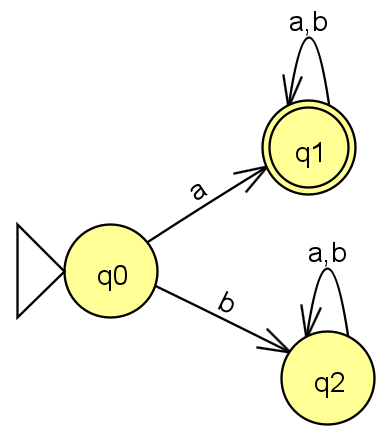
\includegraphics[width=0.2\textwidth]{../../../images/DFAs/ex1_q1.png}



% \vspace{3cm}
% \begin{flushleft}
% أرجو لكم وقتًا ممتعًا.

% الأستاذ محمود اغبارية.
% \end{flushleft}


% \end{document}


\title{ورقة تلخيصية: أساسيات البرمجة كائنية التوجه في \textenglish{C\#} \\ (ما قبل الوراثة)}
\author{أ. محمود اغبارية}

\begin{document}

\maketitle
\thispagestyle{fancy}

%=============================================================
\section{الفصل الأول: بناء الفئات والتعامل مع الكائنات}
%=============================================================

\subsection{مفهوم الفئة والكائن (\textenglish{Class and Object})}
\textbf{الفئة} (\textenglish{Class}) هي قالب أو مخطط مجرد يحدد الخصائص والأساليب. بينما \textbf{الكائن} (\textenglish{Object}) هو نسخة حقيقية تُنشأ من هذا القالب في الذاكرة.
اتفاقيات التسمية (\textenglish{Naming Conventions}): تبدأ أسماء الفئات بحرف كبير (مثل \textenglish{Student}).

\begin{boxExample}
\begin{english}
\begin{minted}{csharp}
class Student
{
    // Attributes
    public string Name;
    public int Age;

    // Methods
    public void PrintInfo()
    {
        Console.WriteLine(Name + " is " + Age + " years old.");
    }
}
\end{minted}
\end{english}
\end{boxExample}

\subsection{إنشاء الكائنات ودالة البناء (\textenglish{Instantiation \& Constructors})}
نستخدم الكلمة \textenglish{new} لإنشاء كائن. وعند الإنشاء يتم استدعاء \textbf{دالة البناء} (\textenglish{Constructor})، وهي دالة خاصة تحمل نفس اسم الفئة وتُستخدم لإعطاء قيم أولية (تهيئة) لخصائص الكائن.

\begin{boxExample}
\begin{english}
\begin{minted}{csharp}
class Student
{
    public string Name;
    public int Age;

    // Default constructor
    public Student()
    {
        Name = "Unknown";
        Age = 0;
    }

    // Parameterized constructor (overloading)
    public Student(string name, int age)
    {
        Name = name;
        Age = age;
    }
}
\end{minted}
\end{english}
\end{boxExample}

\subsection{صيغة النقطة والمتغيرات المرجعية (\textenglish{Dot Notation \& References})}
المتغير الذي يحفظ الكائن هو \textbf{متغير مرجعي} (\textenglish{Reference})، أي أنه يؤشر إلى عنوان الكائن في الذاكرة. للوصول إلى خصائص أو أساليب الكائن، نستخدم \textbf{صيغة النقطة} (\textenglish{Dot Notation}). يتم تمرير الكائنات إلى الدوال كمرجع، مما يعني أن تعديل الكائن داخل الدالة يؤثر على الكائن الأصلي.

\begin{boxExample}
\begin{english}
\begin{minted}{csharp}
Student s1 = new Student("Ahmad", 16);
s1.Age = 17; // Modifying property
s1.PrintInfo(); // Calling method
\end{minted}
\end{english}
\end{boxExample}

\subsection{التحميل الزائد للأساليب (\textenglish{Method Overloading})}
التحميل الزائد يعني كتابة أكثر من دالة بنفس الاسم داخل نفس الفئة، بشرط أن تختلف في عدد أو نوع البارامترات. هذا يتيح مرونة في استدعاء الدالة بحالات مختلفة. رأينا مثالاً على ذلك في دوال البناء المتعددة أعلاه.

\subsection{الكائنات المركبة (\textenglish{Complex Objects})}
يمكن أن تحتوي الفئة على خصائص هي بحد ذاتها كائنات من فئات أخرى.
\begin{boxExample}
\begin{english}
\begin{minted}{csharp}
class Course
{
    public string Title;
    public Student TopStudent; // Complex object
}
\end{minted}
\end{english}
\end{boxExample}

\clearpage
%=============================================================
\section{الفصل الثاني: المفاهيم الهيكلية المتقدمة وتغليف البيانات}
%=============================================================

\subsection{محددات الوصول والتغليف (\textenglish{Access Modifiers \& Encapsulation})}
التغليف (\textenglish{Encapsulation}) يعني إخفاء البيانات الداخلية للفئة وحمايتها من التعديل العشوائي، وتوفير واجهة آمنة للتعامل معها. نستخدم \textenglish{private} لإخفاء الخصائص، و \textenglish{public} للدوال التي تسمح بقراءتها أو تعديلها بأمان.

\begin{boxExample}
\begin{english}
\begin{minted}{csharp}
class BankAccount
{
    private double balance; // Hidden property

    public void Deposit(double amount)
    {
        if (amount > 0)
            balance += amount;
    }

    public double GetBalance()
    {
        return balance;
    }
}
\end{minted}
\end{english}
\end{boxExample}

\subsection{الأعضاء الساكنة (\textenglish{Static Members})}
الأعضاء المعرّفة كـ \textenglish{static} تتبع الفئة نفسها كقالب عام، وليس لكل كائن على حدة. يمكن استدعاؤها مباشرة باستخدام اسم الفئة. من الأمثلة على ذلك فئات الخدمة (\textenglish{Utility Classes}) مثل \textenglish{Math}.

\begin{boxExample}
\begin{english}
\begin{minted}{csharp}
class Calculator
{
    public static int Add(int a, int b)
    {
        return a + b;
    }
}

// Calling without creating an object
int sum = Calculator.Add(5, 3);
\end{minted}
\end{english}
\end{boxExample}

\subsection{المصفوفات ككائنات (\textenglish{Arrays as Objects})}
المصفوفة في \textenglish{C\#} هي كائن، ولها خصائص (مثل \textenglish{Length}) وأساليب. يمكن إنشاء مصفوفات من الكائنات، ويجب الانتباه إلى عدم تجاوز حدود المصفوفة (\textenglish{Out of Bounds}).

\begin{boxExample}
\begin{english}
\begin{minted}{csharp}
Student[] classRoom = new Student[30];
classRoom[0] = new Student("Ali", 16);
Console.WriteLine(classRoom.Length); // Prints 30
\end{minted}
\end{english}
\end{boxExample}

\subsection{فئة النصوص (\textenglish{String Class})}
السلاسل النصية هي كائنات من نوع \textenglish{String}. وهي توفر أساليب مفيدة جداً، وتدعم دمج النصوص. كما يمكننا إعادة تعريف دالة \textenglish{ToString()} في فئاتنا الخاصة لتمثيل الكائن كنص عند طباعته.

\begin{boxExample}
\begin{english}
\begin{minted}{csharp}
class Student
{
    public string Name;
    // Overriding the string representation method
    public override string ToString()
    {
        return "Student Name: " + Name;
    }
}
\end{minted}
\end{english}
\end{boxExample}

\subsection{توثيق الكود واستدعاء الفئات (\textenglish{Documentation \& Using})}
نستخدم الكلمة \textenglish{using} في أعلى الملف لجلب فئات من مساحات أسماء أخرى (\textenglish{Namespaces}). ولتسهيل استخدام الواجهات البرمجية، نستخدم تعليقات التوثيق (\textenglish{XML Docs}) باستخدام ثلاثة خطوط مائلة.

\begin{boxExample}
\begin{english}
\begin{minted}{csharp}
using System;

/// <summary>
/// This class represents a student in a school
/// </summary>
class Student
{
    // ...
}
\end{minted}
\end{english}
\end{boxExample}

\end{document}